\documentclass{article}
\usepackage[utf8]{inputenc}
\usepackage{geometry}
\usepackage{graphicx}
\usepackage{hyperref}


\geometry{
left=25mm,
right=25mm,
top=20mm,
bottom=25mm
}

\title{\textbf{Report N°1 MSc Thesis: Active Constraints}}
\author{\textbf{Alberto Rota} - \textit{Supervisor: Prof. Elena De Momi}}
\date{}

\begin{document}
\maketitle
\paragraph{Title:} \textit{To Be Defined}
\section*{General guidelines}
    Development of surgical training tasks implementing Active Constraints of
    different nature and with different levels of intervention, in order to
    evaluate their efficacy and role in Robot-Assisted Minimally Invasive Sugery.
    % Sviluppo di tasks per surgical training che implementino Active Constraints
    % di diversa tipologia e con differenti livelli di ausilio, per valutarne
    % l'efficacia e il ruolo nella Robot-Assisted Minimally Invasive surgery.
    \begin{itemize}
        \item \textit{Phase 1: }Software Development in a virtual environment (Unity)
        \item \textit{Phase 2: }Implementing on the dVRK, followed by
        experimental tests with data gathering, analysis and validation
        % Applicazione su dVRK seguita da test
        % sperimentali, raccolta e analisi dati, validazione
    \end{itemize}
\section*{Progress}
    In these first weeks of work:
    % In queste prime settimane di lavoro:
    \begin{itemize}
        \item I learned C\# and familiarized better with the Unity Environment 
        % Ho imparato il C\# e familiarizzato meglio con Unity
        \item I selected "Active
        Constraints/Virtual Fixtures: A survey"
        \href{https://ieeexplore.ieee.org/document/6634270}{(link here)} as a
        discrete guide of workflow and as a point of reference on the different
        kinds of Active Constraints and for their implementation on the
        mathematical and software side. 
        % una buona guida per il
        % lavoro e per avere una discreta panoramica sulle diverse tipologie di
        % Virtual Fixtures e della loro implementazione sul lato matematico e
        % Software
        \item From here I creaded a virtual surgical scenario in Unity with the
        model of a Knee as a subject and with the end-effector of a PSM. Inside
        of this virtual scenario: 
        % Da qui ho creato uno scenario chirurgico virtuale in Unity che ha
        % come soggetto un ginocchio e in cui ho inserito l'end-effector di un
        % PSM. All'interno di questo scenario virtuale:
        \begin{itemize}
            \item I implemented the \textit{Trajectory Guidance Active
            Constraints} described in "A Dynamic Non-Energy-Storing 
            Guidance Constraint with Motion 
            Redirection for Robot-Assisted Surgery" \href{https://re.public.polimi.it/retrieve/handle/11311/1008843/167307/A%20Dynamic%20Non-Energy%20Storing%20Guidance.pdf}
            {(link here)}, which functions properly inside the virtual
            surgical scenario
            % Ho implementato il \textit{Trajectory Guidance Active
            % Constraints} descritto in "A Dynamic Non-Energy-Storing 
            % Guidance Constraint with Motion 
            % Redirection for Robot-Assisted Surgery"
            % \href{https://re.public.polimi.it/retrieve/handle/11311/1008843/167307/A%20Dynamic%20Non-Energy%20Storing%20Guidance.pdf}
            % {(link qui)}, che funziona correttamente nella scena chiurgica
            % virtuale
            \item For this same purpose, I also implemented the possibility of
            generating 3D \textit{Hermite Trajectories} starting from any set of
            control points, which are set up in the pre-operatory stage: what is
            described int the previous point has been tested on this kind of
            trajectories
             
            % A tal proposito, ho implementato anche la possibilità di
            % generare \textit{Hermite Trajectories} 3D a partire da control
            % points indivituati in pre-operatorio: quanto implementato sopra è
            % stato testato su trajectories di questo tipo
            \item 
            I implemented the \textit{Surface Avoidance Active
            Constraint} described in "Dynamic 3-D Virtual Fixtures for Minimally
            Invasive Beating Heart Procedures"
            \href{https://ieeexplore.ieee.org/document/4579344}{(link here)},
            which functions properly in the virtual surgical scenario 
            % Ho implementato il \textit{Surface Avoidance Active
            % Constraint} descritto in "Dynamic 3-D Virtual Fixtures for Minimally
            % Invasive Beating Heart Procedures"
            % \href{https://ieeexplore.ieee.org/document/4579344}{(link qui)} che
            % funziona correttamente nella scena chirurgica virtuale
        \end{itemize}
    \end{itemize}
    In the following page I'm showing a few screenshots (and I'm aware of
    their limited descriptiveness) of the virtual surgical scenario with some
    graphic visual aid of what ha been described above.  
    % Nella successiva pagina riporto alcuni screenshot (consapevole della
    % loro limitata descrittività) del \textit{surgical scenario} virtuale.         

\section*{Next Steps}
\begin{itemize}
    \item
    Using "Active Constraints/Virtual Fixtures: A survey" again as a guide,    
    implementing at least one of every kind of virtual fixture described in the
    paper and in the cited and referenced literature (guidance / avoidance / redirection,
    trajectory / surface / volume-based / force-field, static/dynamic, \textit{etc.}).
    % Utilizzando come guida "Active Constraints/Virtual Fixtures: A survey",
    % proseguire nell'implementazione di ognuna delle varie tipologie di Virtual
    % Fixtures esposte (guidance / avoidance / redirection,
    % trajectory / surface / volume-based / force-field, static/dynamic, \textit{etc.}).
    \item 
    Literature research and first implementation (software-wise) of real
    surgical tasks (not limited to surgical training) where to apply the virtual
    fixtures implemented above. 
    % Ricerca in letteratura e prima implementazione di task chirurgiche reali
    % (surgical training e non solo) in cui applicare le Virtual Fixture implementate
\end{itemize}
    
\newpage
\section*{Screenshots}
\begin{figure}[h!]
    \begin{small}
        \begin{center}
            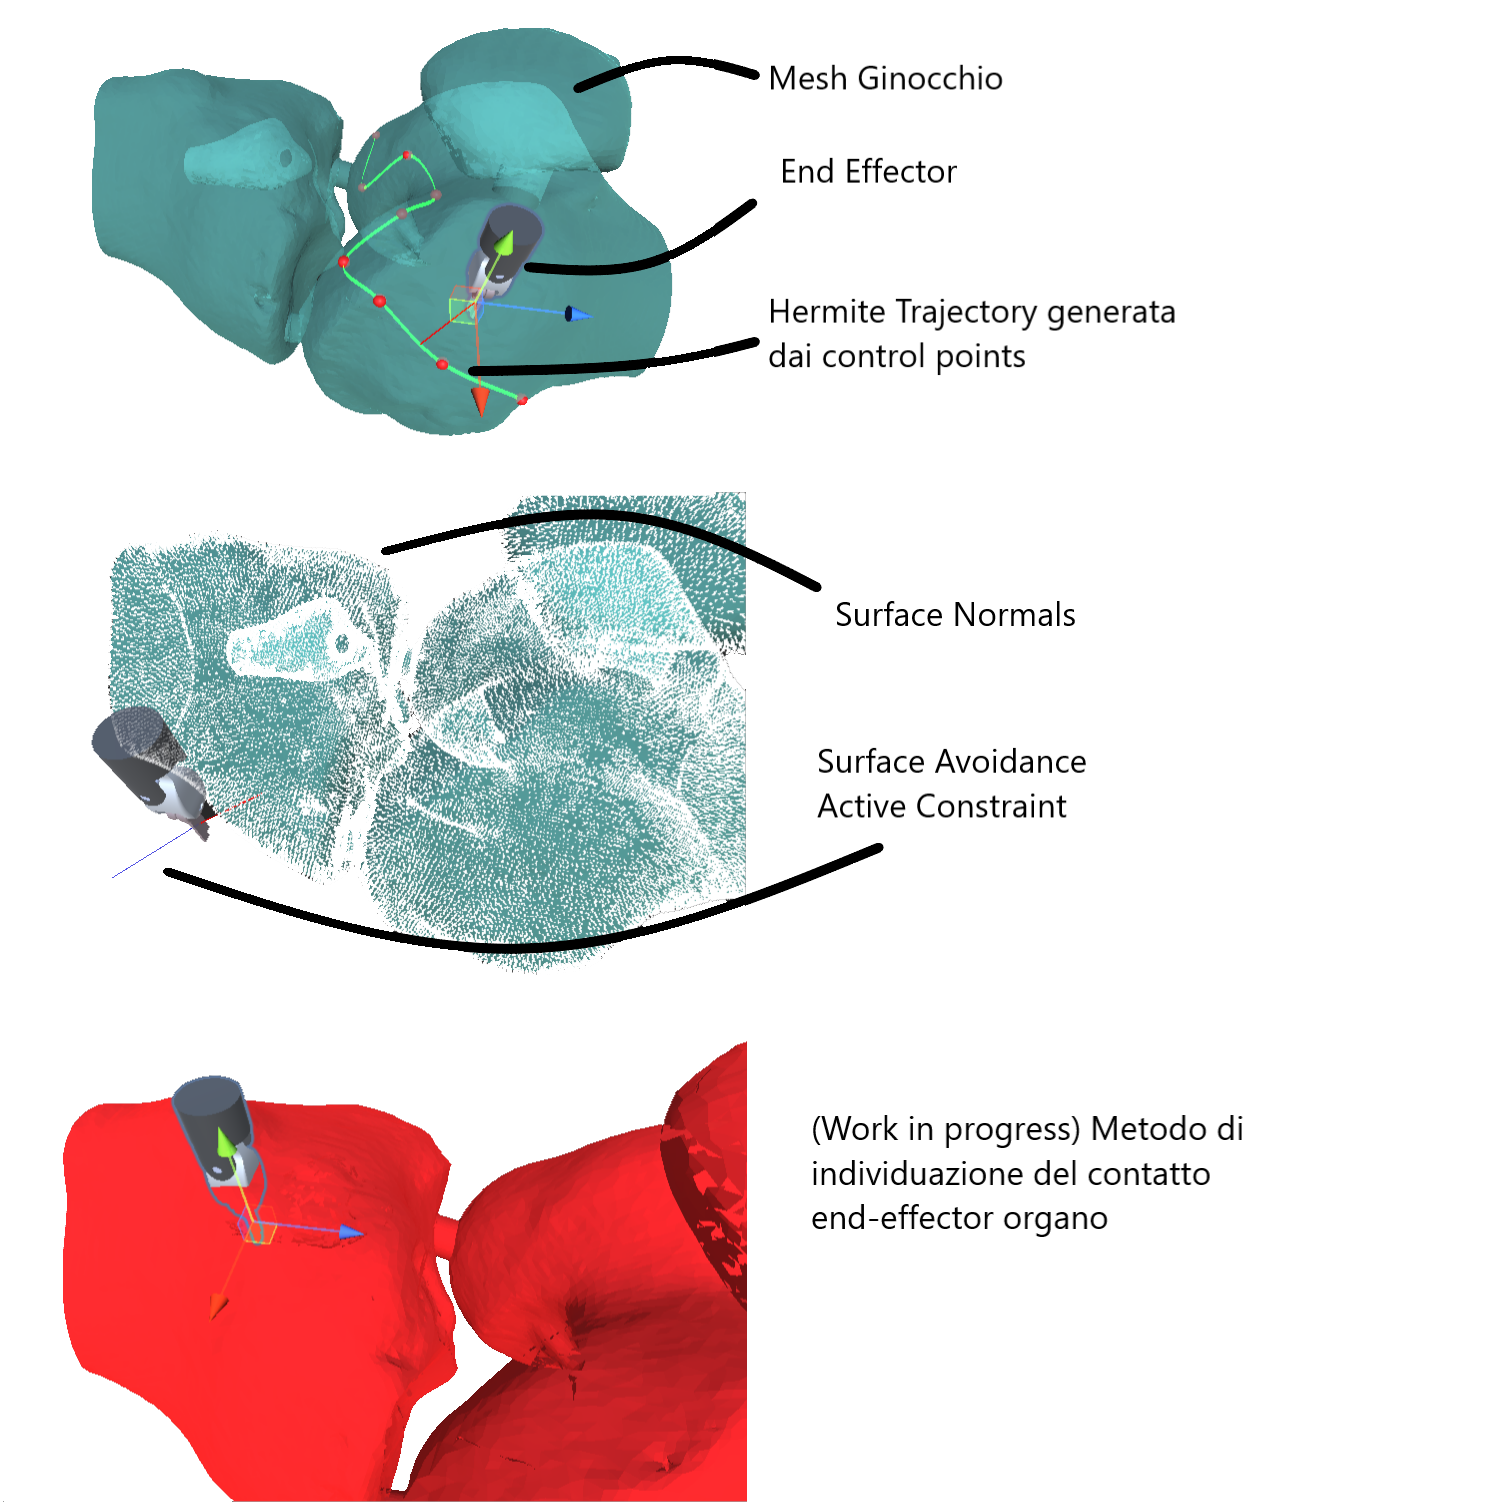
\includegraphics[width=0.95\textwidth]{Scene.png}
        \end{center}[]
        \label{fig:}
    \end{small}
\end{figure}

    
\end{document}